\documentclass[12pt,a4paper]{article}
\usepackage[utf8]{inputenc}
\usepackage[T1]{fontenc}
\usepackage{amsmath,amssymb,amsfonts}
\usepackage{geometry}
\usepackage{listings}
\usepackage{xcolor}
\usepackage{hyperref}
\usepackage{booktabs}
\usepackage{array}
\usepackage{tikz}
\usetikzlibrary{arrows.meta,shapes,positioning,calc}

\geometry{margin=2.5cm}
\lstset{
  basicstyle=\ttfamily\footnotesize,
  keywordstyle=\color{blue!80}\bfseries,
  commentstyle=\color{gray}\itshape,
  stringstyle=\color{red!70},
  breaklines=true,
  frame=single,
  backgroundcolor=\color{gray!5},
  numbers=left,
  numberstyle=\tiny\color{gray},
  captionpos=b
}

\title{\textbf{Report 5: Navigator Module}\\[0.4em]
\large \textbf{Part~I:} Complete Original System --- Every Function\\
\textbf{Part~II:} Every Soaring-Mode Modification and Its Impact\\[0.5em]
\normalsize PX4 Autosoaring Implementation --- Defence Technical Report}
\author{Radhouene --- Fixed-Wing Autosoaring Project}
\date{April 2026}

\begin{document}
\maketitle
\tableofcontents
\newpage

%=============================================================================
\section*{List of Symbols and Acronyms}
\addcontentsline{toc}{section}{List of Symbols and Acronyms}
%=============================================================================

\subsection*{Abbreviations}
\begin{center}\begin{tabular}{ll}\toprule
Symbol & Meaning \\\midrule
NED & North-East-Down coordinate frame \\
AMSL & Above Mean Sea Level \\
uORB & Micro Object Request Broker --- PX4 publish/subscribe IPC \\
GCS & Ground Control Station \\
RTL & Return-To-Launch \\
ADS-B & Automatic Dependent Surveillance--Broadcast (aircraft transponder) \\
VTOL & Vertical Take-Off and Landing \\
NPFG & Nonlinear Path Following Guidance (used by fw\_pos\_control) \\
SP & Setpoint \\
\bottomrule\end{tabular}\end{center}

\subsection*{Key Symbols}
\begin{center}\begin{tabular}{lll}\toprule
Symbol & Meaning & Unit \\\midrule
$(x_c, y_c)$ & Loiter circle centre, NE plane & m \\
$R$ & Loiter circle radius & m \\
$\omega$ & Loiter angular rate & rad/s \\
$V_{\text{TAS}}$ & True airspeed & m/s \\
$h$ & Altitude AMSL & m \\
$h^*$ & Altitude setpoint carried in \texttt{position\_setpoint\_s.alt} & m \\
$r_{\text{acc}}$ & Acceptance radius: distance at which a WP is considered reached & m \\
$r_{\text{alt}}$ & Altitude acceptance radius & m \\
$r_{\text{loiter}}$ & Nominal loiter radius from \texttt{NAV\_LOITER\_RAD} & m \\
$v_{\text{cruise}}$ & Cruising speed setpoint (passed via triplet) & m/s \\
$\delta_t^*$ & Cruising throttle setpoint passed via triplet & --- \\
$d_{\text{geofence}}$ & Look-ahead test-point distance for geofence check & m \\
\bottomrule\end{tabular}\end{center}

\subsection*{Key uORB Topics}
\begin{center}\begin{tabular}{lll}\toprule
Topic & Direction & Content \\\midrule
\texttt{position\_setpoint\_triplet} & Published & Previous / current / next WP setpoints \\
\texttt{mission\_result} & Published & Mission validity, current WP index \\
\texttt{navigator\_status} & Published & Active navigation mode, geofence status \\
\texttt{vehicle\_roi} & Published & Region-of-interest target for camera/gimbal \\
\texttt{vehicle\_command\_ack} & Published & Acknowledgement of handled commands \\
\texttt{vehicle\_local\_position} & Subscribed (fd) & Local NED position and velocity \\
\texttt{vehicle\_global\_position} & Subscribed & Global lat/lon/alt \\
\texttt{vehicle\_status} & Subscribed (fd) & Nav state, arming state, vehicle type \\
\texttt{vehicle\_command} & Subscribed & Commands from Commander, GCS, pos\_ctrl \\
\texttt{mission} & Subscribed (fd) & Mission item list \\
\texttt{home\_position} & Subscribed & Home lat/lon/alt \\
\texttt{land\_detected} & Subscribed & Landed / in-air state \\
\texttt{position\_controller\_status} & Subscribed & Bearing, acceptance radius from FW/MC pos ctrl \\
\texttt{gps\_position} & Subscribed & Raw GPS for geofence check \\
\texttt{transponder\_report} & Subscribed (ADS-B) & Other aircraft positions \\
\bottomrule\end{tabular}\end{center}

\subsection*{Navigation Modes Owned by Navigator}
\begin{center}\begin{tabular}{ll}\toprule
Object & Mode \\\midrule
\texttt{\_mission} (\texttt{Mission}) & AUTO\_MISSION: follows waypoint list \\
\texttt{\_loiter} (\texttt{Loiter}) & AUTO\_LOITER: circles a fixed point \\
\texttt{\_rtl} (\texttt{RTL}) & AUTO\_RTL: return to home \\
\texttt{\_takeoff} (\texttt{Takeoff}) & AUTO\_TAKEOFF \\
\texttt{\_land} (\texttt{Land}) & AUTO\_LAND \\
\texttt{\_precland} (\texttt{PrecLand}) & AUTO\_PRECLAND \\
\texttt{\_vtol\_takeoff} (\texttt{VtolTakeoff}) & AUTO\_VTOL\_TAKEOFF \\
\bottomrule\end{tabular}\end{center}

\subsection*{MAVLink Commands Handled by Navigator's run()}
\begin{center}\begin{tabular}{ll}\toprule
Command ID & Purpose \\\midrule
\texttt{DO\_REPOSITION} (192) & Move the loiter centre, optionally switch to LOITER \\
\texttt{DO\_CHANGE\_ALTITUDE} (186) & Change loiter altitude \\
\texttt{DO\_ORBIT} (34) & GCS-commanded circular orbit \\
\texttt{DO\_FIGUREEIGHT} (35) & Figure-eight pattern (FW only) \\
\texttt{NAV\_TAKEOFF} (22) & Set takeoff position \\
\texttt{NAV\_VTOL\_TAKEOFF} (84) & VTOL takeoff position \\
\texttt{DO\_LAND\_START} (189) & Jump to land sequence in mission \\
\texttt{MISSION\_START} (300) & Jump to specific mission item \\
\texttt{DO\_CHANGE\_SPEED} (178) & Override cruising speed/throttle \\
\texttt{DO\_SET\_ROI} (201) & Set region of interest \\
\texttt{DO\_GO\_AROUND} (23) & Acknowledge go-around (handled by pos ctrl) \\
\texttt{DO\_VTOL\_TRANSITION} (3000) & Reset speed/throttle on VTOL transition \\
\bottomrule\end{tabular}\end{center}

\newpage
%=============================================================================
\part{Original Navigator System}
%=============================================================================

%=============================================================================
\section{Module Purpose and Architecture}
%=============================================================================

The \texttt{navigator} module is the \textbf{position setpoint manager} of PX4.
It sits between the Commander (which decides the navigation \emph{state}) and the
position controllers (which track the setpoints).

\begin{center}
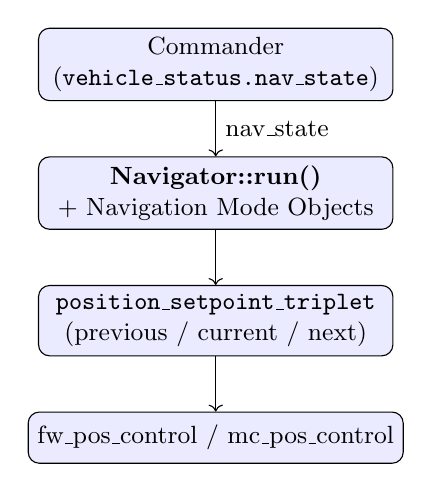
\begin{tikzpicture}[node distance=1.3cm,
  box/.style={draw,rounded corners,fill=blue!8,minimum width=4.5cm,
              minimum height=0.65cm,align=center,font=\small}]
  \node[box] (cmd) {Commander\\(\texttt{vehicle\_status.nav\_state})};
  \node[box,below=0.7cm of cmd] (nav) {\textbf{Navigator::run()}\\+ Navigation Mode Objects};
  \node[box,below=0.7cm of nav] (tri) {\texttt{position\_setpoint\_triplet}\\(previous / current / next)};
  \node[box,below=0.7cm of tri] (pos) {fw\_pos\_control / mc\_pos\_control};
  \draw[->] (cmd) -- (nav) node[midway,right,font=\small] {nav\_state};
  \draw[->] (nav) -- (tri);
  \draw[->] (tri) -- (pos);
\end{tikzpicture}
\end{center}

\textbf{Key invariant:} Navigator never issues attitude or throttle commands.
It only produces a \texttt{position\_setpoint\_triplet\_s} containing:
\begin{itemize}
  \item \texttt{previous}: last visited waypoint (for cross-track error computation).
  \item \texttt{current}: active waypoint/loiter centre.
  \item \texttt{next}: look-ahead waypoint (for smooth trajectory).
\end{itemize}

%=============================================================================
\section{Navigator() Constructor}
%=============================================================================

\begin{lstlisting}[language=C++]
Navigator::Navigator()
\end{lstlisting}

Runs once at module start:
\begin{enumerate}
  \item Creates the performance counter \texttt{\_loop\_perf}.
  \item Constructs all navigation mode objects, passing \texttt{this} as the
        parent navigator:
        \texttt{\_mission(this)}, \texttt{\_loiter(this)}, \texttt{\_rtl(this)},
        \texttt{\_takeoff(this)}, \texttt{\_land(this)},
        \texttt{\_precland(this)}, \texttt{\_vtol\_takeoff(this)}.
  \item Fills \texttt{\_navigation\_mode\_array[]} with pointers to all modes.
  \item Calls \texttt{initialize()} on every navigation mode (sets each to idle).
  \item Caches parameter handles:
        \texttt{VT\_B\_DEC\_MSS}, \texttt{MPC\_JERK\_AUTO}, \texttt{MPC\_ACC\_HOR}
        (used by RTL and path planning).
  \item Opens three file-descriptor subscriptions:
        \texttt{vehicle\_local\_position},
        \texttt{mission},
        \texttt{vehicle\_status}.
  \item Advertises and initialises the
        \texttt{distance\_sensor\_mode\_change\_request} topic (requests
        distance sensor on/off as needed by landing modes).
  \item Calls \texttt{reset\_triplets()} to mark all setpoints invalid.
\end{enumerate}

%=============================================================================
\section{params\_update()}
%=============================================================================

\begin{lstlisting}[language=C++]
void Navigator::params_update()
\end{lstlisting}

Called on startup and whenever \texttt{parameter\_update} is received.
\begin{itemize}
  \item \texttt{updateParams()} --- reads all \texttt{DEFINE\_PARAMETERS} from
        the module's parameter list (acceptance radii, loiter radius,
        RTL settings, geofence action, etc.).
  \item Reads parameter handles for VTOL deceleration, MPC jerk, and MPC
        acceleration (these are not in the navigator's own parameter list but
        are shared with other modules).
  \item Sets the mission command timeout:
        \texttt{\_mission.set\_command\_timeout(\_param\_mis\_command\_tout.get())}.
  \item On ADS-B builds: updates conflict detection parameters.
\end{itemize}

%=============================================================================
\section{run() --- The Main Control Loop}
%=============================================================================

\subsection{Startup (once)}
\begin{enumerate}
  \item Try to load geofence from \texttt{/fs/microsd/etc/geofence.txt}.
  \item Call \texttt{params\_update()}.
  \item Set up three \texttt{poll()} file descriptors:
        \texttt{\_local\_pos\_sub} (50\,ms rate-limit),
        \texttt{\_vehicle\_status\_sub},
        \texttt{\_mission\_sub}.
\end{enumerate}

\subsection{Per-Cycle Steps}

The loop calls \texttt{px4\_poll()} with a 1000\,ms timeout.

\paragraph{1. Copy sensor data.}
Every iteration:
\begin{itemize}
  \item \texttt{orb\_copy(vehicle\_local\_position)} $\to$ \texttt{\_local\_pos}.
  \item \texttt{orb\_copy(vehicle\_status)} $\to$ \texttt{\_vstatus}.
  \item If mission fd active: copy mission, update geofence/safe-points if IDs changed.
  \item If GPS updated: copy \texttt{\_gps\_pos}.
  \item If global position updated: copy \texttt{\_global\_pos}.
\end{itemize}

\paragraph{2. Parameter update.}
If \texttt{\_parameter\_update\_sub.updated()}: call \texttt{params\_update()}.

\paragraph{3. Auxiliary subscriptions.}
\begin{itemize}
  \item \texttt{\_land\_detected\_sub.update(\&\_land\_detected)}.
  \item \texttt{\_position\_controller\_status\_sub.update()}.
  \item \texttt{\_home\_pos\_sub.update(\&\_home\_pos)}.
\end{itemize}

\paragraph{4. Vehicle command processing.}
Up to \texttt{ORB\_QUEUE\_LENGTH} commands per cycle, but only when
\texttt{\_wait\_for\_vehicle\_status\_timestamp == 0}
(the wait mechanism prevents overwriting a reposition setpoint before the
vehicle status has been refreshed after a mode switch):
\begin{enumerate}
  \item Copy the command.
  \item Dispatch to the appropriate handler (see Section~\ref{sec:commands}).
\end{enumerate}

\paragraph{5. ADS-B traffic check (if compiled in).}
\texttt{check\_traffic()} reads transponder reports and, on conflict,
calls \texttt{take\_traffic\_conflict\_action()}.

\paragraph{6. Geofence breach check.}
\texttt{geofence\_breach\_check()} (Section~\ref{sec:geofence}).

\paragraph{7. Navigation mode state machine.}
Maps \texttt{\_vstatus.nav\_state} to a \texttt{NavigatorMode*}
(Section~\ref{sec:navmode}).

\paragraph{8. Triplet reset on mode switch.}
If \texttt{\_navigation\_mode != navigation\_mode\_new}: reset the triplet,
\emph{unless} switching from takeoff to loiter with a valid loiter point
(to preserve the takeoff altitude).

\paragraph{9. VTOL descend-to-hover override.}
If \texttt{nav\_state == NAVIGATION\_STATE\_DESCEND}, vehicle is VTOL, and
currently fixed-wing, and \texttt{force\_vtol()} is true: send
\texttt{DO\_VTOL\_TRANSITION} to transition back to multi-copter.

\paragraph{10. Run all navigation modes.}
Iterate \texttt{\_navigation\_mode\_array[]}; call \texttt{mode.run(active)}
for each. Only the active mode computes new setpoints; inactive modes receive
\texttt{run(false)} (housekeeping only).

\paragraph{11. Handle null mode (no active navigation).}
If \texttt{\_navigation\_mode == nullptr}: publish an invalid triplet once.

\paragraph{12. Publish outputs.}
\begin{itemize}
  \item If \texttt{\_pos\_sp\_triplet\_updated}: call
        \texttt{publish\_position\_setpoint\_triplet()}.
  \item If \texttt{\_mission\_result\_updated}: call
        \texttt{publish\_mission\_result()}.
  \item Always: \texttt{publish\_navigator\_status()}.
  \item Always: \texttt{publish\_distance\_sensor\_mode\_request()}.
  \item Always: \texttt{\_geofence.run()} (geofence logic tick).
\end{itemize}

%=============================================================================
\section{Vehicle Command Handlers in run()}
\label{sec:commands}
%=============================================================================

\subsection{VEHICLE\_CMD\_DO\_REPOSITION (192)}

This is the most complex command handler. It is \emph{only} executed when
the vehicle is armed.

\paragraph{Wait mechanism.}
Before processing, a wait timestamp is set:
\begin{lstlisting}[language=C++]
_wait_for_vehicle_status_timestamp = hrt_absolute_time();
\end{lstlisting}
This prevents the next command from overwriting the reposition setpoint before
Commander has processed the matching mode-switch command.

\paragraph{Position resolution.}
\begin{equation}
  \texttt{lat} = \begin{cases}
    \texttt{cmd.param5} & \text{if finite} \\
    \texttt{\_global\_pos.lat} & \text{otherwise (hover at current position)}
  \end{cases}
\end{equation}
Same for longitude. Altitude:
\begin{equation}
  \texttt{alt} = \begin{cases}
    \texttt{cmd.param7} & \text{if finite} \\
    \texttt{\_global\_pos.alt} & \text{otherwise}
  \end{cases}
\end{equation}

\paragraph{Geofence check.}
If the resolved position is outside the active geofence:
reject with MAVLink log message; do \textbf{not} update the triplet.

\paragraph{Triplet construction (if inside geofence).}
\begin{enumerate}
  \item \texttt{rep->previous} $\leftarrow$ current vehicle position
        (yaw, lat, lon, alt, timestamp).
  \item \texttt{rep->current.type = SETPOINT\_TYPE\_LOITER}.
  \item Ground speed: if \texttt{param1 > 0 and finite}: use \texttt{param1};
        else use default \texttt{get\_cruising\_speed()} (or $-1$ on loiter entry).
  \item \texttt{rep->current.cruising\_throttle = get\_cruising\_throttle()}.
  \item \texttt{rep->current.acceptance\_radius = get\_acceptance\_radius()}.
  \item Yaw: \texttt{param4} if finite, else NaN.
  \item Position logic:
        \begin{itemize}
          \item If \texttt{param5} and \texttt{param6} both finite:
                full position change.
          \item Else if only \texttt{param7} or \texttt{param4} finite:
                altitude/yaw-only change (keep current loiter lat/lon).
          \item Else (all NaN): pause vehicle.
                Fixed-wing: loiter at current position.
                Rotary-wing: pre-project stop point.
        \end{itemize}
  \item Altitude-only change branch: copy current loiter radius, minor radius,
        orientation, and pattern from the active setpoint.
  \item \textbf{Radius and direction (original code):}
        \begin{lstlisting}[language=C++]
// ORIGINAL:
if (PX4_ISFINITE(cmd.param3) && cmd.param3 > 0) {
    rep->current.loiter_radius = cmd.param3; // always positive
    // direction: never changed from param3
}
        \end{lstlisting}
  \item Mark setpoint valid, set timestamps.
  \item \texttt{\_time\_loitering\_after\_gf\_breach = 0}.
\end{enumerate}

\subsection{VEHICLE\_CMD\_DO\_CHANGE\_ALTITUDE (186)}

Identical to \texttt{DO\_REPOSITION} with only altitude changed.
Only \texttt{param1} (altitude AMSL) is used; lat/lon kept from current setpoint.
Geofence check is also performed.

\subsection{VEHICLE\_CMD\_DO\_ORBIT (34) --- Fixed-Wing}

For fixed-wing only (multicopter handles orbits in flight tasks):
\begin{itemize}
  \item \texttt{param1}: signed radius (negative = counter-clockwise).
  \item \texttt{param5/6/7}: loiter centre lat/lon/alt.
  \item Type: \texttt{LOITER\_TYPE\_ORBIT}.
\end{itemize}
Geofence check applied.

\subsection{VEHICLE\_CMD\_DO\_FIGUREEIGHT (35) --- Fixed-Wing}

\begin{itemize}
  \item \texttt{param2}: minor radius of the figure-eight.
  \item \texttt{param1}: major radius (default: $2.5 \times$ minor radius).
  \item \texttt{param4}: orientation angle of the figure-eight axis.
  \item Pattern: \texttt{LOITER\_TYPE\_FIGUREEIGHT}.
\end{itemize}
Major radius enforced $\geq 2 \times$ minor radius.

\subsection{VEHICLE\_CMD\_NAV\_TAKEOFF (22)}

Stores the takeoff setpoint in \texttt{\_takeoff\_triplet}:
\begin{itemize}
  \item Previous: current vehicle position (if home position valid).
  \item Current type: \texttt{SETPOINT\_TYPE\_TAKEOFF}.
  \item Lat/lon: from \texttt{param5/6} if valid, else current position.
  \item Alt: \texttt{param7}.
  \item Yaw: NaN (handled by FlightTaskAuto).
  \item Speed: $-1$ (reset to default).
\end{itemize}

\subsection{VEHICLE\_CMD\_DO\_LAND\_START (189)}

Looks up the \texttt{NAV\_CMD\_DO\_LAND\_START} item in the mission.
If found, sends \texttt{VEHICLE\_CMD\_MISSION\_START} with the index of the next
position-setpoint item after the land-start item.

\subsection{VEHICLE\_CMD\_MISSION\_START (300)}

Calls \texttt{\_mission.set\_current\_mission\_index(param1)}.
This causes the mission mode object to advance the active waypoint.

\subsection{VEHICLE\_CMD\_DO\_CHANGE\_SPEED (178)}

\begin{itemize}
  \item If \texttt{param2 > 0}: \texttt{set\_cruising\_speed(param2)}.
  \item Else: \texttt{reset\_cruising\_speed()}.
        If \texttt{param3 > 0}: \texttt{set\_cruising\_throttle(param3/100)}.
\end{itemize}
Acknowledged immediately with ACCEPTED.

\subsection{VEHICLE\_CMD\_DO\_SET\_ROI variants (201, 202, 195, 197, 198)}

Builds and publishes \texttt{vehicle\_roi\_s}:
\begin{center}\begin{tabular}{ll}\toprule
Command & ROI mode \\\midrule
\texttt{DO\_SET\_ROI} / \texttt{NAV\_ROI} & Uses \texttt{param1} as mode \\
\texttt{DO\_SET\_ROI\_LOCATION} & Fixed lat/lon/alt from \texttt{param5/6/7} \\
\texttt{DO\_SET\_ROI\_WPNEXT\_OFFSET} & Offset from next waypoint (pitch/roll/yaw) \\
\texttt{DO\_SET\_ROI\_NONE} & Clears ROI \\
\bottomrule\end{tabular}\end{center}

%=============================================================================
\section{Navigation Mode State Machine}
\label{sec:navmode}
%=============================================================================

After command processing, the mode is resolved:

\begin{center}\begin{tabular}{ll}\toprule
\texttt{nav\_state} & Navigator object \\\midrule
\texttt{NAVIGATION\_STATE\_AUTO\_MISSION} & \texttt{\_mission} \\
\texttt{NAVIGATION\_STATE\_AUTO\_LOITER} & \texttt{\_loiter} \\
\texttt{NAVIGATION\_STATE\_AUTO\_RTL} & \texttt{\_rtl} (unless already landing) \\
\texttt{NAVIGATION\_STATE\_AUTO\_TAKEOFF} & \texttt{\_takeoff} \\
\texttt{NAVIGATION\_STATE\_AUTO\_VTOL\_TAKEOFF} & \texttt{\_vtol\_takeoff} \\
\texttt{NAVIGATION\_STATE\_AUTO\_LAND} & \texttt{\_land} \\
\texttt{NAVIGATION\_STATE\_AUTO\_PRECLAND} & \texttt{\_precland} \\
MANUAL / ACRO / ALTCTL / POSCTL / etc.\ & \texttt{nullptr} (no navigator output) \\
\bottomrule\end{tabular}\end{center}

\textbf{Disarmed guard:} If \texttt{arming\_state != ARMED}: force
\texttt{navigation\_mode\_new = nullptr} regardless of nav\_state.

\textbf{RTL exception:} If already in mission and landing
(\texttt{\_mission.isLanding()}): stay in mission mode; do not switch to RTL.

\textbf{All six mode objects run every cycle}, but only the active one
generates setpoints. Inactive modes receive \texttt{run(false)} for
internal housekeeping (e.g.\ resetting state machines).

%=============================================================================
\section{The Position Setpoint Triplet}
%=============================================================================

\subsection{Structure: position\_setpoint\_s}

Each setpoint in the triplet carries:
\begin{center}\begin{tabular}{ll}\toprule
Field & Meaning \\\midrule
\texttt{lat, lon, alt} & 3-D target position (WGS-84 / AMSL) \\
\texttt{type} & IDLE / POSITION / VELOCITY / LOITER / TAKEOFF / LAND / FOLLOW\_TARGET \\
\texttt{yaw} & Target heading (NaN = don't care) \\
\texttt{loiter\_radius} & Circle radius for loiter [m] \\
\texttt{loiter\_direction\_counter\_clockwise} & true = CCW, false = CW \\
\texttt{loiter\_pattern} & ORBIT / FIGUREEIGHT \\
\texttt{loiter\_minor\_radius} & Semi-minor radius for figure-eight \\
\texttt{loiter\_orientation} & Figure-eight axis angle [rad] \\
\texttt{acceptance\_radius} & Waypoint acceptance sphere radius [m] \\
\texttt{alt\_acceptance\_radius} & Altitude acceptance band [m] \\
\texttt{cruising\_speed} & Override speed for this leg ($-1$ = default) [m/s] \\
\texttt{cruising\_throttle} & Override throttle for this leg (NaN = default) \\
\texttt{valid} & Whether this setpoint should be used \\
\texttt{timestamp} & hrt time [us] \\
\bottomrule\end{tabular}\end{center}

\subsection{publish\_position\_setpoint\_triplet()}

\begin{lstlisting}[language=C++]
void Navigator::publish_position_setpoint_triplet()
{
    _pos_sp_triplet.timestamp = hrt_absolute_time();
    _pos_sp_triplet_pub.publish(_pos_sp_triplet);
    _pos_sp_triplet_updated = false;
}
\end{lstlisting}

Called whenever \texttt{\_pos\_sp\_triplet\_updated} is true.
The consumer (\texttt{fw\_pos\_control}) polls this topic and rebuilds its
NPFG / TECS inputs on every new triplet.

\subsection{reset\_triplets() and reset\_position\_setpoint()}

\begin{lstlisting}[language=C++]
void Navigator::reset_triplets()
{
    reset_position_setpoint(_pos_sp_triplet.previous);
    reset_position_setpoint(_pos_sp_triplet.current);
    reset_position_setpoint(_pos_sp_triplet.next);
    _pos_sp_triplet_updated = true;
}
\end{lstlisting}

\texttt{reset\_position\_setpoint(sp)} fills a setpoint with safe defaults:
\begin{itemize}
  \item \texttt{lat = lon = NaN}, \texttt{yaw = NaN}.
  \item \texttt{loiter\_radius = get\_loiter\_radius()} (from \texttt{NAV\_LOITER\_RAD}).
  \item \texttt{acceptance\_radius = get\_default\_acceptance\_radius()} (from \texttt{NAV\_ACC\_RAD}).
  \item \texttt{cruising\_speed = get\_cruising\_speed()}.
  \item \texttt{cruising\_throttle = get\_cruising\_throttle()}.
  \item \texttt{valid = false}, \texttt{type = SETPOINT\_TYPE\_IDLE}.
  \item \texttt{loiter\_direction\_counter\_clockwise = false} (clockwise default).
\end{itemize}

%=============================================================================
\section{Acceptance Radius Functions}
%=============================================================================

\subsection{get\_default\_acceptance\_radius()}
Returns \texttt{\_param\_nav\_acc\_rad.get()} = \texttt{NAV\_ACC\_RAD} (default 10\,m).
Used for horizontal waypoint acceptance.

\subsection{get\_altitude\_acceptance\_radius()}

Vehicle-type dependent:
\begin{center}\begin{tabular}{lll}\toprule
Vehicle type & Condition & Returns \\\midrule
Fixed-wing & \texttt{curr\_sp.alt\_acceptance\_radius} valid & That value \\
Fixed-wing & Next sp is LAND and not force-VTOL & \texttt{NAV\_FW\_ALTL\_RAD} (tighter, before landing) \\
Fixed-wing & Otherwise & \texttt{NAV\_FW\_ALT\_RAD} \\
Rover & Any & $\infty$ (altitude not used) \\
Rotary-wing & Any & \texttt{NAV\_MC\_ALT\_RAD} (or from current sp) \\
\bottomrule\end{tabular}\end{center}

\subsection{get\_acceptance\_radius()}
Returns $\max(\texttt{NAV\_ACC\_RAD},\; \texttt{pos\_ctrl\_status.acceptance\_radius})$
for fixed-wing and rover (NPFG provides its own switch-distance).
For multicopter: returns \texttt{NAV\_ACC\_RAD}.

%=============================================================================
\section{Cruising Speed and Throttle}
%=============================================================================

\subsection{get\_cruising\_speed()}
Returns \texttt{\_mission\_cruising\_speed} if set by a mission item
(\texttt{NAV\_CMD\_DO\_CHANGE\_SPEED}), otherwise returns $-1$ (use aircraft default).

\subsection{get\_cruising\_throttle()}
Returns \texttt{\_mission\_throttle} if set by a mission
\texttt{DO\_CHANGE\_SPEED} with \texttt{param3 > 0}, otherwise NaN
(use \texttt{FW\_THR\_TRIM}).

\subsection{set\_cruising\_speed() / reset\_cruising\_speed()}
Set/clear \texttt{\_mission\_cruising\_speed}.

\subsection{set\_cruising\_throttle() / reset}
Set/clear \texttt{\_mission\_throttle}.

%=============================================================================
\section{Geofence Breach Check}
\label{sec:geofence}
%=============================================================================

\begin{lstlisting}[language=C++]
void Navigator::geofence_breach_check()
\end{lstlisting}

Runs at \texttt{GEOFENCE\_CHECK\_INTERVAL\_US} = 200\,ms when a geofence is active.

\paragraph{Test-point computation.}

The check is performed at a \emph{look-ahead} point in the current direction of
travel to give the aircraft time to react:

\begin{center}\begin{tabular}{lll}\toprule
Vehicle type & Test-point distance $d_{\text{geofence}}$ & Source \\\midrule
Rotary-wing & Braking distance from current velocity & \texttt{GFBreachAvoidance} model \\
Fixed-wing & $2 r_{\text{loiter}}$ & Conservative fixed radius \\
\bottomrule\end{tabular}\end{center}

\paragraph{Geofence action (configurable via \texttt{GF\_ACTION}):}

\begin{center}\begin{tabular}{ll}\toprule
\texttt{GF\_ACTION} & Response \\\midrule
0 = NONE & Ignored \\
1 = WARN & MAVLink warning only \\
2 = LOITER & Switch to LOITER, loiter for \texttt{GF\_MAX\_HOR\_DIST} \\
3 = RTL & Trigger RTL \\
4 = TERMINATE & Flight termination \\
5 = LAND & Immediate landing \\
\bottomrule\end{tabular}\end{center}

If a geofence breach is detected and action $\geq$ LOITER: the navigator publishes
a \texttt{geofence\_result} topic and sets the failsafe trigger.

%=============================================================================
\section{publish\_navigator\_status()}
%=============================================================================

Publishes \texttt{navigator\_status\_s} every cycle:
\begin{itemize}
  \item \texttt{nav\_state}: current navigator mode (mirrors \texttt{vehicle\_status.nav\_state}).
  \item \texttt{failure\_type}: geofence/traffic/etc.\ failure.
  \item \texttt{timestamp}.
\end{itemize}

%=============================================================================
\section{abort\_landing()}
%=============================================================================

\begin{lstlisting}[language=C++]
bool Navigator::abort_landing()
\end{lstlisting}

Returns true if:
\begin{itemize}
  \item The current setpoint type is \texttt{SETPOINT\_TYPE\_LAND}; AND
  \item A fresh \texttt{position\_controller\_landing\_status} has been
        received with \texttt{abort\_status > 0} (e.g.\ ground slope too steep,
        terrain hold timeout).
\end{itemize}
Used by the \texttt{Land} navigation mode to abort an approach.

%=============================================================================
\section{ADS-B Traffic Handling}
%=============================================================================

\begin{lstlisting}[language=C++]
void Navigator::check_traffic()
\end{lstlisting}

If a new transponder report has the required validity flags
(coordinates, heading, velocity, altitude):
\begin{enumerate}
  \item \texttt{\_adsb\_conflict.detect\_traffic\_conflict()}: checks relative
        geometry using configurable horizontal/vertical separation thresholds.
  \item If conflict detected: \texttt{take\_traffic\_conflict\_action()} issues
        RTL / land / loiter depending on \texttt{NAV\_TRAFF\_AVOID}.
  \item Stale conflicts removed after timeout.
\end{enumerate}

%=============================================================================
\section{Other Utility Functions}
%=============================================================================

\begin{center}\begin{tabular}{lll}\toprule
Function & Returns & Notes \\\midrule
\texttt{get\_loiter\_radius()} & \texttt{NAV\_LOITER\_RAD} & Default loiter radius [m] \\
\texttt{force\_vtol()} & bool & True for VTOL FW in descend mode (needs hover) \\
\texttt{get\_yaw\_to\_be\_accepted(yaw)} & bool & True if yaw is finite \\
\texttt{load\_fence\_from\_file()} & void & Delegates to \texttt{\_geofence.loadFromFile()} \\
\texttt{publish\_vehicle\_command()} & void & Re-publishes a command for internal routing \\
\texttt{publish\_vehicle\_command\_ack()} & void & Sends \texttt{vehicle\_command\_ack} \\
\texttt{acquire\_gimbal\_control()} & void & Sends gimbal-manager-take-control \\
\texttt{release\_gimbal\_control()} & void & Releases gimbal control \\
\texttt{stop\_capturing\_images()} & void & Camera-trigger stop command \\
\texttt{disable\_camera\_trigger()} & void & Disables camera trigger mode \\
\texttt{set\_gimbal\_neutral()} & void & Centres gimbal \\
\texttt{mode\_completed()} & void & Called by navigation mode on completion \\
\texttt{set\_mission\_failure\_heading\_timeout()} & void & Triggers mission failure timer \\
\texttt{trigger\_hagl\_failsafe()} & void & Height-above-ground failsafe event \\
\texttt{sendWarningDescentStoppedDueToTerrain()} & void & MAVLink warning \\
\texttt{preproject\_stop\_point()} & void & For multicopter, projects a braking stop point \\
\texttt{geofence\_allows\_position()} & bool & True if global position is inside geofence \\
\bottomrule\end{tabular}\end{center}

%=============================================================================
\part{Soaring-Mode Modifications}
%=============================================================================

%=============================================================================
\section{Overview of Changes}
%=============================================================================

Two changes were made to Navigator for soaring:
\begin{enumerate}
  \item The \texttt{DO\_REPOSITION} handler was extended to support a
        \textbf{signed radius} convention for loiter direction.
  \item The \texttt{NAVIGATION\_STATE\_ORBIT} nav state was mapped to
        \texttt{\_loiter} in the navigation mode state machine.
\end{enumerate}
All other Navigator functionality is \textbf{unchanged}.

%=============================================================================
\section{Modification N1: Signed Radius in DO\_REPOSITION}
%=============================================================================

\subsection{Physical Background: Loiter Direction}

For a circular loiter of radius $R$ centred at $(x_c, y_c)$ in the NED
North-East plane, the aircraft's position at time $t$ is:
\begin{equation}
  \begin{pmatrix} x(t) \\ y(t) \end{pmatrix}
  = \begin{pmatrix} x_c \\ y_c \end{pmatrix}
  + R \begin{pmatrix} \cos(\omega t + \phi_0) \\ \sin(\omega t + \phi_0) \end{pmatrix}
\end{equation}

where $\phi_0$ is the initial phase angle and the angular rate is:
\begin{equation}
  \omega = \frac{V_{\text{TAS}}}{R} \quad [\text{rad/s}]
\end{equation}

In the NED (North-East-Down) frame:
\begin{equation}
  \omega = \begin{cases}
    +\dfrac{V_{\text{TAS}}}{R} & \text{counter-clockwise (positive)} \\[6pt]
    -\dfrac{V_{\text{TAS}}}{R} & \text{clockwise (negative)}
  \end{cases}
\end{equation}

PX4 uses the boolean field
\texttt{loiter\_direction\_counter\_clockwise} in \texttt{position\_setpoint\_s}
to encode this. The default is \texttt{false} (clockwise).

\subsection{Original Parsing}

\begin{lstlisting}[language=C++]
// ORIGINAL CODE in navigator_main.cpp
if (PX4_ISFINITE(cmd.param3) && cmd.param3 > 0) {
    rep->current.loiter_radius = cmd.param3;  // always positive
    // loiter_direction_counter_clockwise: never changed from param3
}
\end{lstlisting}

\textbf{Consequence:}
\begin{itemize}
  \item Negative \texttt{param3} values were silently ignored (the condition
        \texttt{param3 > 0} rejected them).
  \item There was no way to command CCW loiter via \texttt{DO\_REPOSITION}.
  \item Direction was always the navigator default (clockwise).
\end{itemize}

\subsection{Modified Parsing}

\begin{lstlisting}[language=C++]
// MODIFIED CODE
// Convention:
//   param3 > 0  --> clockwise   (loiter_direction_counter_clockwise = false)
//   param3 < 0  --> counter-clockwise (loiter_direction_counter_clockwise = true)
//   param3 == 0 or NaN --> use NAV_LOITER_RAD default, keep direction
if (PX4_ISFINITE(cmd.param3) && fabsf(cmd.param3) > FLT_EPSILON) {
    rep->current.loiter_radius = fabsf(cmd.param3);
    rep->current.loiter_direction_counter_clockwise = (cmd.param3 < 0.f);

} else if (!only_alt_change_requested) {
    rep->current.loiter_radius = get_loiter_radius();
    // direction stays at navigator default (false = CW)
}
\end{lstlisting}

\textbf{Key change:}
\begin{itemize}
  \item The condition changed from \texttt{param3 > 0} to
        \texttt{fabsf(param3) > FLT\_EPSILON} --- accepts both positive
        and negative values.
  \item \texttt{loiter\_radius} is now set to the absolute value
        \texttt{fabsf(cmd.param3)} (always positive, as required by the
        loiter controller).
  \item \texttt{loiter\_direction\_counter\_clockwise} is set from the sign:
        \begin{equation}
          \texttt{CCW} = (\texttt{param3} < 0)
        \end{equation}
\end{itemize}

\subsection{Encoding in FixedwingPositionControl}

The companion-side caller builds the signed radius before publishing
\texttt{DO\_REPOSITION}:

\begin{lstlisting}[language=C++]
// In FixedwingPositionControl::control_auto()
const float sign = _autosoaring_control.loiter_clockwise ? 1.f : -1.f;
cmd.param3 = sign * R_eff;   // signed: + = CW, - = CCW
\end{lstlisting}

The direction semantics are thus:
\begin{center}\begin{tabular}{lll}\toprule
\texttt{loiter\_clockwise} & \texttt{cmd.param3} & Navigator result \\\midrule
\texttt{true} (CW) & $+R_{\text{eff}}$ & \texttt{loiter\_direction\_CCW = false} \\
\texttt{false} (CCW) & $-R_{\text{eff}}$ & \texttt{loiter\_direction\_CCW = true} \\
\bottomrule\end{tabular}\end{center}

\subsection{Direction-Change Re-Trigger Logic}

The loiter direction is \emph{not} re-applied automatically when the
companion changes direction; the navigator only processes new
\texttt{DO\_REPOSITION} commands. Therefore, \texttt{fw\_pos\_control} must
re-send \texttt{DO\_REPOSITION} when the direction changes even if the
position is unchanged:

\begin{lstlisting}[language=C++]
// In FixedwingPositionControl::control_auto()
const bool direction_changed =
    (_autosoaring_control.loiter_clockwise != _soaring_last_clockwise);
const bool pos_changed =
    (first_activation && airspeed_ok_for_thermal)
    || explicit_pos_changed
    || direction_changed;  // new: re-send even if only direction changed

if (pos_changed) {
    // ... build and publish DO_REPOSITION with new signed radius
    _soaring_last_clockwise = _autosoaring_control.loiter_clockwise;
}
\end{lstlisting}

\texttt{\_soaring\_last\_clockwise} is latched after each command to prevent
re-sending on every cycle.

%=============================================================================
\section{Modification N2: ORBIT Nav State Maps to Loiter Mode}
%=============================================================================

\subsection{Original Behaviour}

In the original code, \texttt{NAVIGATION\_STATE\_ORBIT} was not present in the
navigation mode switch. It fell through to the \texttt{default} case, which
set \texttt{navigation\_mode\_new = nullptr}. The navigator produced no setpoints
in ORBIT state, effectively freezing the aircraft.

\subsection{Modified Behaviour}

\begin{lstlisting}[language=C++]
case vehicle_status_s::NAVIGATION_STATE_ORBIT:
    // Thermal loiter: reuse the loiter navigation mode.
    // The companion selects the centre via DO_REPOSITION;
    // we simply map this nav-state to the existing loiter handler.
    _pos_sp_triplet_published_invalid_once = false;
    navigation_mode_new = &_loiter;
    break;
\end{lstlisting}

\textbf{Why ORBIT?}
The standard GCS orbit command (\texttt{DO\_ORBIT}) sets
\texttt{nav\_state = NAVIGATION\_STATE\_ORBIT} via Commander.
By mapping ORBIT to \texttt{\_loiter}, the soaring thermal mode can exploit
the same orbit-request path as a standard GCS orbit command, re-using the
mature loiter navigation mode without any new mode object.

\subsection{Impact}

\begin{itemize}
  \item When the companion sends \texttt{soaring\_mode = 3 (THERMAL\_LOITER)},
        \texttt{fw\_pos\_control} sends \texttt{DO\_REPOSITION} which causes
        Commander to switch to \texttt{NAVIGATION\_STATE\_AUTO\_LOITER}
        (the primary path). The ORBIT mapping is a safety net for the case
        where a GCS sends \texttt{DO\_ORBIT} directly.
  \item No existing loiter functionality is affected; the loiter mode object
        \texttt{\_loiter} processes either LOITER or ORBIT nav states
        identically.
\end{itemize}

%=============================================================================
\section{Interaction Diagram: Full Thermal Loiter Flow}
%=============================================================================

\begin{center}
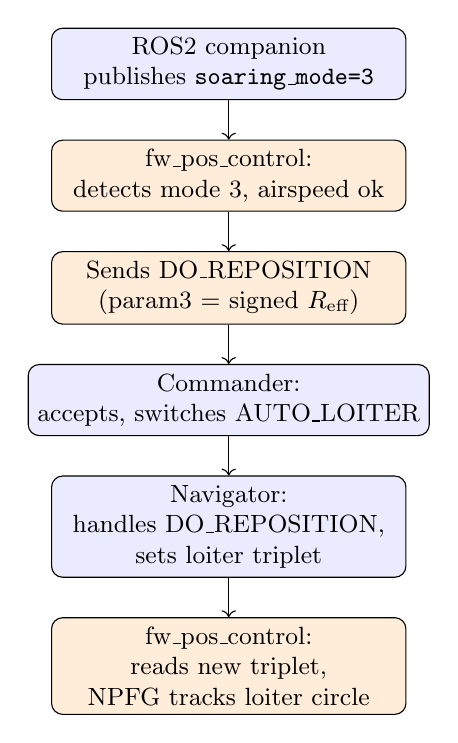
\begin{tikzpicture}[node distance=1.2cm,
  box/.style={draw,rounded corners,fill=blue!8,minimum width=4.5cm,
              minimum height=0.65cm,align=center,font=\small},
  act/.style={draw,rounded corners,fill=orange!15,minimum width=4.5cm,
              minimum height=0.65cm,align=center,font=\small}]
  \node[box] (ros) {ROS2 companion\\publishes \texttt{soaring\_mode=3}};
  \node[act,below=0.5cm of ros] (fwpc1) {fw\_pos\_control:\\detects mode 3, airspeed ok};
  \node[act,below=0.5cm of fwpc1] (cmd1) {Sends DO\_REPOSITION\\(param3 = signed $R_{\text{eff}}$)};
  \node[box,below=0.5cm of cmd1] (comm) {Commander:\\accepts, switches AUTO\_LOITER};
  \node[box,below=0.5cm of comm] (nav) {Navigator:\\handles DO\_REPOSITION,\\ sets loiter triplet};
  \node[act,below=0.5cm of nav] (fwpc2) {fw\_pos\_control:\\reads new triplet,\\NPFG tracks loiter circle};
  \draw[->] (ros) -- (fwpc1);
  \draw[->] (fwpc1) -- (cmd1);
  \draw[->] (cmd1) -- (comm);
  \draw[->] (comm) -- (nav);
  \draw[->] (nav) -- (fwpc2);
\end{tikzpicture}
\end{center}

\noindent\textit{Note:} when the operator stops soaring via CLI (\texttt{soar:off}),
\texttt{fw\_pos\_control} publishes \texttt{autosoaring\_status} (ROS\,2:
\texttt{/fmu/out/autosoaring\_status}) for the companion; this does not add new
Navigator commands (see Report~1 and Report~3).

%=============================================================================
\section{Summary Table: All Modifications to Navigator}
%=============================================================================

\begin{center}\begin{tabular}{p{3.5cm}p{4.5cm}p{5cm}}\toprule
Aspect & Original & Modified \\\midrule
\texttt{DO\_REPOSITION} radius condition & \texttt{param3 > 0} only & \texttt{fabsf(param3) > epsilon} (positive or negative) \\
\texttt{DO\_REPOSITION} direction & Always default (CW) & Sign of \texttt{param3}: $+$ = CW, $-$ = CCW \\
\texttt{NAVIGATION\_STATE\_ORBIT} & \texttt{nullptr} (no setpoints) & Maps to \texttt{\_loiter} object \\
Direction-change re-send & Not supported & \texttt{direction\_changed} flag in fw\_pos\_control re-triggers \texttt{DO\_REPOSITION} \\
\bottomrule\end{tabular}\end{center}

\end{document}
